\section{Data and methodology}
\label{sec:method}

The search looks for one kind of signal: an unresolved carrier at the star's
own position, narrow compared with a single correlator channel, and drifting in
sky frequency because the transmitter accelerates along the line of sight. Over
a long track its power is spread across many channels, so a search that treats
each channel on its own will miss it. The analysis therefore \emph{de-drifts}
the data before it measures them. It shifts each integration's spectrum to
follow a trial drift rate and only then adds them together.

\subsection{The de-drifted search statistic}
\label{sec:statistic}

Each window's dynamic spectrum is stacked along every trial drift rate
$\dot\nu$. The search statistic is the largest stacked signal-to-noise
ratio anywhere on the resulting channel$\times$drift grid,
%
\begin{equation}
T(\mathbf{x})=\max_{\dot\nu,\;\nu}\;
\frac{\sum_{t} I\!\left(\mathbf{x},t,\nu+\dot\nu t\right)
       \big/\sigma^{2}(t,\nu+\dot\nu t)}
     {\left[\sum_{t}1\big/\sigma^{2}(t,\nu+\dot\nu t)\right]^{1/2}},
\label{eq:tstar}
\end{equation}
%
where $I(\mathbf{x},t,\nu)$ is the spectrum at sky position $\mathbf{x}$
in integration $t$ and channel $\nu$, and $\sigma(t,\nu)$ is the noise scale
there. Both weights are evaluated at the channel the track occupies in that
integration, $\nu+\dot\nu t$, and not at the channel that labels it. Equation~\ref{eq:tstar} is the inverse-variance-weighted stack of the
calibrated intensities along a constant-drift track, divided by the nominal
noise of that stack. It is the matched filter for such a carrier, and $T$ an
absolute signal-to-noise ratio, only when the noise is independent between
integrations and between channels, an idealisation for which no optimality is
claimed. The trigger is therefore set against the distribution $T$ takes in
the data, given empirically in every window by \NCtrl{} control positions on
the same visibilities and through the same stack, so any correlation the noise
carries is inside them; and a value of $T$ is converted into a power by
injected carriers recovered through the unchanged pipeline
(\S\ref{sec:pninetysel}), without passing through the independence assumption
at all. In Equation~\ref{eq:tstar} the time $t$ runs from the first integration of the
observation, so the frequency $\nu$ that labels a track is the one a carrier
would occupy at the start of that block, and a repeat epoch is read at the
cell the same convention fixes (\S\ref{sec:etacrv}).
The noise scale is the median absolute deviation
across \NCtrl{} control positions at each integration and each channel,
scaled to its Gaussian-equivalent standard deviation: local in time and
frequency, global in position, and shared by the star and every control.
They lie, from a fixed seed, in an annulus set by each block's own
synthesised and primary beams: the field read over is that block's primary
beam.
The statistic is evaluated at one position at a time, identically at the
star and at each control, which is what makes the two comparable.
$T_\star$ denotes its value at the star.

Spectra are extracted at the star's apparent position, never from images: for
each integration and each native channel the pipeline forms the weighted vector
average of the phase-shifted visibilities in total intensity, the mean
$I=(XX+YY)/2$ of the two parallel-hand correlations. That average is the
dirty-map value at the extraction position -- an amplitude, not a deconvolved
flux density, so not a point-source measurement where the field holds extended
emission -- and the correction for its displacement is measured with
carriers injected into the same visibilities, not assumed
(Appendix~\ref{app:pbresp}). The data are the archive's calibrated deliveries
with two exceptions. ALMA's pipeline and online flags were not applied:
recalibrating \FgNEbMeas{} blocks with them takes \FgNCrossFallWord{} of the
\FgNCrossMeas{} crossings tested below the trigger, every one unattributed and
without a recurrence or in the block failing the quality criterion, and makes
the limits of the affected blocks up to \FgLimDeepMaxPct{} per cent too deep,
the deepest limit unchanged. And the flux-scaling step was not run on the
\LgNEbFluxWord{} blocks calibrated by legacy scripts, which are up to
\LgFluxMaxPct{} per cent too bright. Every
delivered channel is searched, with no regridding, deconvolution or edge trimming;
a per-integration median along the \emph{frequency} axis removes the
continuum, a level and not a shape, and no median is taken along time, so no
feature narrow against the band can be removed by it. The
delivered channels are smoothed, so flux density times channel width is not
yet a radiated power; a response correction computed from the correlator's
own channel shape supplies the difference (Appendix~\ref{app:conventions}).

One convention holds everywhere in the paper. The search runs on the
topocentric sky frequencies ALMA delivered, and every drift rate quoted is the
apparent one at the telescope, which is what the data contain and what a reader
can recompute from the archived channel axes. Two steps need the star's own
frame: a crossing is compared with the line catalogue, and a repeat epoch is
read at the \emph{predicted cell}. That cell is the single channel at a single
drift rate where the first epoch's own fit says a carrier should be. Both steps
take the star's frame by correcting each block's frequency axis for the
Earth's motion at that epoch and then for the star's systemic velocity. That
velocity is the catalogued radial velocity from SIMBAD \citep{SIMBAD2000},
queried on \SimbadQueryDate, and zero where none exists --
\FrZeroVsysClause{} (Section~\ref{sec:sample}). One star departs: toward $\beta$~Pic the
adopted value is \BpRecVsys\,km\,s$^{-1}$, the stellar radial velocity adopted
in the ALMA CO analysis of its disk \citep{Matra2017}. This survey's own
blocks reproduce it. It exceeds the catalogued value by about the
template-mismatch offset the \textit{Gaia} pipeline documents for stars this
hot \citep{Blomme2023}.

Two power quantities carry the main text, both defined in
Table~\ref{tab:quantities}: the trigger level $P_{\rm trig} = 4\pi
d^{2}S\,\Delta\nu$ at distance $d$, for a carrier that makes $T_\star$ reach
$T_{\rm trig}=\StageNullTrig$ in one native channel of width $\Delta\nu$, and
the sensitivity $\mathrm{EIRP}_{90}$, measured by injecting synthetic carriers
of known amplitude into calibrated visibilities and recovering them through
the unmodified pipeline (\S\ref{sec:pninetysel}). Every limit quoted in this
paper is the $\mathrm{EIRP}_{90}$ of its own window, given to two significant
figures beside its native channel width, except the bare-threshold comparisons
of \S\ref{sec:intro} and Fig.~\ref{fig:context}(a), which are labelled as
such; its error budget is Table~\ref{tab:p90budget}. The amplitude scale is
checked twice: an independent reduction of the same AU~Mic visibilities is
reproduced to \PxJanRatio\,$\pm$\,\PxJanRatioErr, which tests the extraction
and not ALMA's flux transfer, and the published quiescent flux density of
$\epsilon$~Eridani is recovered to \PxEpsRatio\,$\pm$\,\PxEpsRatioErr{}
\citep{Burton2022}, which measures the scale to \SbEpsPct{} per cent. The
absolute scale is therefore carried at ALMA's own band-dependent accuracy
specification: $\pm\BudComb$ per cent for the sample as a whole and
$\pm\BudCombWorst$ for the \BudNHiWin{} Class~A windows in
\BudHiBandWord~\BudHiBands, at \BudHiGHzList\,GHz.

The drift range searched is bounded by an acceleration, not by a frequency.
Drift rate and line-of-sight acceleration are one quantity in two sets of
units,
%
\begin{equation}
\frac{\dot\nu}{\nu}=\frac{a_{\rm los}}{c}
\qquad\text{and so}\qquad
a_{\rm los}=\frac{c\,\dot\nu}{\nu},
\label{eq:accel}
\end{equation}
%
so a ceiling expressed as $\dot\nu/\nu$ is the same physical limit in every
band. The default ceiling is \DriftCeilLo--\DriftCeilHi\,Hz\,s$^{-1}$\,GHz$^{-1}$,
the acceleration of a transmitter orbiting a solar-type star at a few
hundredths of an au. That is the \citet{Mason2025} fiducial with a threefold
margin, and \AccelSheikhPct{} per cent of the \AccelSheikhNHz\,nHz that
\citet{Sheikh2019} recommend for a general search. The ceiling is widened for
a confirmed exoplanet host whenever the innermost known planet demands more. As an acceleration it is
\AccelCeilMed\,m\,s$^{-2}$, the median over the Class~A windows, rising to
\AccelCeilMax\,m\,s$^{-2}$ on the \AccelNWide{} \AccelWideStar{} windows; the
grid is uniform in $\dot\nu$, fine enough that a carrier midway between two
trials loses no more than \DriftGridFineHalf{} of a native channel over the
longest track, and runs from the negative ceiling to the first trial at or
beyond the positive one, the largest measured
\EgTopMeasAAcc\,m\,s$^{-2}$ (Appendix~\ref{sec:edge}).
\textbf{The survey does not constrain a transmitter whose apparent acceleration
exceeds that range}, and three cases put one there. The first is a
deliberately chirped carrier, which is in any case not distinguished from an
accelerating platform. The second is a transmitter not bound to a known
planet. The third is the sum of orbital and rotational acceleration, which
share the one budget, so a transmitter on a rapidly rotating planet can exceed
the ceiling on its spin alone. $\beta$~Pictoris~b, the fastest rotation measured for any planetary-mass object
and orbiting one of the stars searched here, corresponds to
\AccelBpicRotNHz\,nHz \citep{Sheikh2019}. For the most demanding known case,
transiting TRAPPIST-1~b, \TrapPhaseHi{} per cent of the orbital phase lies
above the default ceiling. Its maximum line-of-sight acceleration equals
the widened grid used on that star's own windows to within the
$\pm\TrpAmaxPct$ per cent its host's mass and orbit are known to. The
fraction of phase above that grid is therefore anywhere between nothing and a sixth
(Fig.~\ref{fig:accel}).

\begin{figure}
\centering
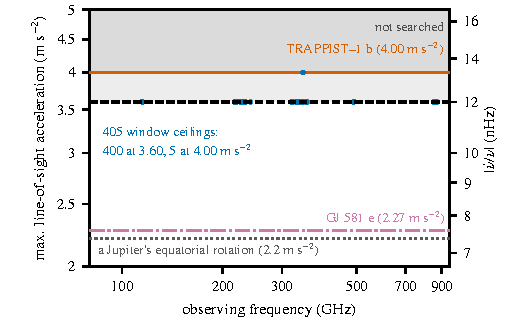
\includegraphics[width=\columnwidth]{figures/drift_acceleration.pdf}
%% ★★★ v4.26 (r25-captions): 11 PRINTED LINES -> R1 §7's limit of about six.
%% TEN macros had this caption as their ONLY citation site -- \AccelCeilMed,
%% \AccelCeilMax, \AccelNWide, \AccelWideStar, \AccelWorstName,
%% \AccelSecondName, \AccelWorstVal, \AccelSecondVal, \AccelJupRot,
%% \AccelJupPct -- so every one of those clauses had to MOVE and none could
%% be deleted: retire_macros.py would otherwise have taken ten numbers out of
%% the paper without a gate going red.  They are now two sentences of
%% \S\ref{sec:statistic} above, beside the ceiling they qualify.  The caption
%% keeps what reads the panel: what a point is, both axes, the shading, and
%% that the horizontal lines are reference accelerations.
\caption{What the drift search reaches, as a physical selection function: the
drift ceiling of each of the \NWinA{} Class~A windows (points), by
Equation~\ref{eq:accel}, against observing frequency, with the unsearched
region shaded and the same quantity as a fractional drift rate on the right.
Horizontal lines are the reference accelerations of \S\ref{sec:statistic}.}
\label{fig:accel}
\end{figure}

Only part of the archive can carry a drift search at all: the maximum searched
drift must cross of order one channel or more over the on-source track,
$\eta_{\rm drift} = |\dot\nu_{\max}|\tau_{\rm track}/\Delta\nu_{\rm ch}
\gtrsim 1$. \EtaDriftAOk{} of the \NWinA{} Class~A windows satisfy it and
\EtaDriftALo{} fall below, in every case because the track is short and not
because the channel is coarse; the released per-window catalogue carries
$\eta_{\rm drift}$ for every window. \EtaDriftBHi{} of the \NWinB{} coarse
windows meet the criterion and stay in Class~B, because meeting it is
necessary for drift discrimination and not sufficient
(Table~\ref{tab:quantities}); all of their systems already carry fine-channel
coverage and none of the \EtaDriftBHi{} holds a crossing.

\subsection{From a crossing to a confirmed signal}
\label{sec:summary}

Every window passes through the same three steps in the same order -- the
trigger, the line attribution and the recurrence test -- and what comes out of
them is a \emph{crossing}, an \emph{unattributed crossing} and, had one
survived, a \emph{confirmed signal}, each defined in
Table~\ref{tab:quantities} and used in no other sense. None of the three is a
significance test. Every count reported below is read from the ledger, which
lists every crossing the search produced, including those in the archival-tail
blocks and in the quality-failing block. The counts are of primary crossings,
one to a window; the \CkNSecondary{} secondary crossings of
\S\ref{sec:technosearch} pass through the same steps, \CkNSecUnattrWord{}
reaching the second and none the third.

\emph{The trigger.} The level on $T_\star$ carries no tail probability, since
$T$ is not shown to follow any standard distribution under the null, and a
window holds between \TuCellsLo{} and $\TuCellsHi$ channel$\times$drift
cells, so one level buys very different protection in a coarse single-pointing
window and in a finely channelised one on a long track. Every cell that
reaches it is recorded, not only the largest in each window, because a carrier
is masked as effectively by a noise excursion as by a line.

\emph{The background.} Because a fixed threshold is not a fixed false-alarm
rate, the number of crossings expected by chance is computed window by window
from the exceedance rate at that window's own control positions, and the
reserved blocks test the one assumption this makes, that a star behaves like a
control position in its own field (\S\ref{sec:trigunif}); a crossing in them
is reported regardless, since a transmitter there would matter whatever its
calibration role. The comparison needs each block's control ensemble to behave
like noise, and one block, \BqFailBlock{} toward \BqFailStar, fails the
criterion of Appendix~\ref{sec:blockquality}. It holds \BqFailNCross{} of the
\NCross{} crossings, the survey's entire Class~B crossing population, all in
coarse-channel windows, so the Class~A results are identical with it and
without it, and the quality-passing data hold \EvNCrossQp{} crossings, all of
them Class~A. \BkFlagNCrossOther{} of those lies in a window the same
diagnostic flags inside a passing block; it is counted, and withheld from the
amplitude-dependent tests where each is made. The \CkNCrossCenA{} in the
primary census are the baseline every expectation is set against, the
\CeNTailCrossWord{} in archival-tail blocks enter none, and the failing
block's \BqFailNCross{} are reported in the ledger and not as crossings of the
same standing (Appendix~\ref{app:falsealarm}). Three corrections precede
the statistic: the extraction field is chosen so that the star lies inside the
delivered primary-beam field and not merely inside the quoted field of view;
the stellar position is propagated to the observation epoch for proper motion,
though not for the annual parallax or for orbital motion, whose omissions are
corrected window by window in \S\ref{sec:pninetysel} and bounded for every
component of a multiple in Appendix~\ref{app:pbresp}; and on-source time is
accounted per integration from the delivered exposure records and not from the
scan intentions.

Two diagnostics attach to the second step, and each says which crossing
deserves attention first without deciding anything. The first ranks $T_\star$
against the same statistic at the window's \NCtrl{} control positions, none of
which sits on the star; its lowest value, $1/(\NCtrl+1)$, means the star beat
every control. It is a ranking filter and not a significance test, because the
stellar and control positions are not demonstrably exchangeable: the annulus
responds to whatever it surrounds, and no parameter-free correction for its
geometry restores an exchangeable statistic (Appendix~\ref{app:radius}).
Weighted star by star, because the five largest stars of the reserved set
carry \BkRankTopFiveWin{} of its \HoWin{} windows, the census median rank is
\BkRankBalSurv{} (\BkRankBalSurvLo--\BkRankBalSurvHi) and the reserved
blocks' \BkRankBalHo{} (\BkRankBalHoLo--\BkRankBalHoHi), both consistent with
the one half exchangeability implies. The rank responds to compactness and
not to origin: genuine carbon monoxide toward $\beta$~Pictoris ranks below its
own control ring, because the resolved disc lifts the ring with the star. The
second diagnostic, a visibility-domain fit, asks whether a crossing's emission
is at the stellar coordinates, but it cannot discriminate at the trigger
either, because at that level a noise maximum at the star fits as a point
source there (\S\ref{sec:vistest}). Neither gates a disposition, so neither is
charged to the sensitivity. Throughout, $p$ denotes a genuine significance
level, and no probability computed against the rank's own null is called one.

\emph{The line attribution} is a single database query, made on \MkListDate{}
and repeatable as it stands, and its $\pm\MaskHalfKms$\,km\,s$^{-1}$
half-width follows the Keplerian line-of-sight velocities of gas surviving
beyond a few au with margin for the systemic velocity; a crossing inside it,
in the star's own rest frame, is \emph{attributed} where the species is one
that such systems are known to carry, and a further \SoNCrossWord{} crossings
coincide with a species no debris disc has been shown to carry, whose offsets
are reported and which are counted as unattributed
(Appendix~\ref{app:linemask}). Halving the half-width leaves the split unchanged:
\FrAttrWTwentyFive{} attributed and \FrUnattrWTwentyFive{} unattributed at
$\pm25$\,km\,s$^{-1}$, against \FrAttrWFifty{} and \FrUnattrWFifty{} at
$\pm\MaskHalfKms$\,km\,s$^{-1}$. A coincidence is a statement about a catalogue and not a
property of a frequency, so an attribution is not a disposal: all \CnCross{}
crossings go on to the recurrence test whichever side of the mask they fall,
and the price of the mask is that the survey constrains nothing inside it.

\emph{The recurrence test.} One reason covers both halves of
\emph{separated}: blocks of one session share calibrators, atmosphere,
correlator setup and interference environment, and the residual of
\S\ref{sec:bdblock} is what that can produce, which holds for two blocks of
one session however far apart they were executed -- \QfNPairDrop{} pairs of
blocks here are of one session and more than a day apart, the widest by
\QfSameSessMaxD\,d. So a recovery in any block of the discovery's own
session is a \emph{within-session repeat} whatever the interval, and no number
of them makes a confirmation; this is also the rule the confirmability census
of \S\ref{sec:mmdifferent} scores the archive on. What a confirmation
requires, and the two readings that test it, are defined in
Table~\ref{tab:quantities}. It is a weak criterion, and the archive's uneven
temporal sampling is why: only part of the sample has epochs separated well
enough to apply it at all.

That the chain finds what it is meant to find is shown twice over, by the
injected carriers of \S\ref{sec:pninetysel} and by $\beta$~Pictoris CO -- a
real feature at a known stellar position, recovered and localised in two
transitions and \CsBpCoBlocks{} execution blocks (\S\ref{sec:bpicval}).

%% (Comment blocks carried forward verbatim from the paragraphs this
%% section consolidated; they print nothing.)
%% ★★★★ FIG. 4 (the detection chain, chain_v412.pdf) IS REMOVED, on Referee
%% 1-4.3's own test: Table~\ref{tab:quantities} defines the three levels and
%% \S\ref{sec:technosearch} gives every count the figure drew, so the figure
%% carried nothing of its own.  0.31 pp of float area and a 5-line caption.
%% ► Its 13 lines of internal small print were ALSO the subject of three
%%   separate referee requests -- show 54 + 2 rather than all 56 against the
%%   census, take the word "excluded" off it, and cut the small print to three
%%   lines -- and none of the three arises once it is gone.
%% ►► MUST LAND WITH THIS: `make_fig_chain_v412.py` retired from
%%   `make_all.sh` and `figures/chain_v412.pdf` deleted, or `figorphan.py`
%%   clause (2) fails on a figure built and included nowhere.  Two retirement
%%   comments for earlier chain figures (v403, v411) are already in
%%   `make_all.sh` and this one belongs beside them.
%% ► \CnCross, \CkNSecondary and \CkNSecUnattrWord were moved out of this
%%   caption into \S\ref{sec:summary}'s paragraph in the previous round so
%%   that deleting it could not take three counts out of the paper in
%%   silence; all three are still cited there and in \S\ref{sec:technosearch}.
%% ► To restore the figure, revert this comment block and the \ref in the
%%   paragraph above; the generator is still in the repository.
%% ★★ v4.26 (r25-captions), FLAGGED AND REPAIRED, NOT INTRODUCED HERE.  This
%% sentence reached the built PDF as "...because a noise maxi-mum at the the
%% star (S4.5)." -- a doubled article AND a clause with no verb, so the
%% duplicated word was the only visible sign that something had been lost.
%% Removing the duplicate alone would have hidden the fragment instead of
%% fixing it.  The completion asserts nothing new: that the fit cannot tell a
%% noise maximum at the star from a source there at the trigger level is what
%% the first half of this same sentence says and what \S\ref{sec:vistest}
%% measures ("the fit excludes neither crossing: injected sources in the bin
%% these two occupy return Re/sigma = ...").  ►► IF THE ORIGINAL CLAUSE CAN BE
%% RECOVERED FROM AN EARLIER VERSION, PREFER IT TO THIS.
%% This heading said "and a rule fixed in advance says so", which the paper then
%% contradicts two appendices later: the condition was noticed in one block and
%% the criterion written afterwards.  The honest version says what the rule is
%% and leaves its provenance to the place that states it, so the two passages
%% cannot disagree.

\begin{table*}
\centering
\caption{The quantities and the three words this paper uses, defined once.
Every term below is used in this sense throughout and in no other. The
distinction the first three rows draw is the one the limits of
\S\ref{sec:pninetysel} turn on: a crossing is a single-epoch event, and a
confirmed signal needs a second and separated epoch that no sensitivity
supplies.}
\label{tab:quantities}
\small
\begin{tabular}{@{}p{0.145\textwidth}p{0.825\textwidth}@{}}
\hline
Term & Definition \\
\hline
Crossing &
A channel\,$\times$\,drift cell at the stellar position reaching
$T_\star\geq\StageNullTrig$ in one execution block; neighbouring channels
above the trigger belong to one crossing. The largest in a window is its
\emph{primary} crossing and any other a \emph{secondary} one, and because the
largest cell is the window's own statistic a secondary crossing exists only
where a primary one does. An event requiring investigation; no claimed
significance. \\
Unattributed crossing &
A crossing lying more than $\MaskHalfKms$\,km\,s$^{-1}$ in the star's frame
from every transition of the line catalogue. That is a reproducible frequency
coincidence; which coincidences are astrophysically plausible is a separate
judgement, stated with each one. A target for follow-up; not a detection. \\
Confirmed signal &
The same carrier found again in a \emph{separated} block -- a different
observing session, more than \EpSep{} day from the discovery -- at a
frequency one bounded trajectory inside the drift grid joins to the
discovery. Two readings test that, and they are not the same test. The
\emph{line-recurrence check} is the operational one: it reads the single
channel and drift the discovery predicts in the star's frame, so it recovers
only a carrier that comes back to that cell, within $\pm\RqDvLo$ to
$\pm\RqDvHi$\,km\,s$^{-1}$ -- which is what a spectral line does and an
accelerating carrier need not. It is applied to every crossing with a covering
repeat block, attributed or not, and a null there is a statement about
attribution and never an exclusion; \MkAttrRecur{} line-attributed crossings pass it,
this stage's positive control (\S\ref{sec:etacrv}). The \emph{trajectory
comparison} searches the $\pm\WdHalfKms$\,km\,s$^{-1}$ about that cell and
asks whether one bounded trajectory joins two crossings; it is the reading
that bears on a drifting carrier. It separates \TjNExcl{} of the \TjNPair{}
pairs and has never accepted a drifting carrier, so a pair it cannot separate
is \emph{open}: neither a confirmation nor an exclusion
(Table~\ref{tab:pairs}). Neither reading exists unless the archive covered
the frequency again in a separated block, and for \ZcNoRepSys{} Class~A
systems it never did, so no sensitivity makes a confirmed signal possible
there. \\
$P_{\rm trig}$ &
The power of a carrier that makes $T_\star$ reach the trigger in one native
channel. An internal pipeline level: not a sensitivity, not a
significance. \\
$\mathrm{EIRP}_{90}$ &
The power at which nine injected carriers in ten produce a crossing at the
star: a measured single-epoch trigger completeness, not a detection
probability. Measured for the \SensNInj{} injected Class~A windows; for the
other \SensNTransfer{} an estimate from the class-average calibration,
interpolated within the injected configurations for \NgNInterpWin{} and
extrapolated beyond them for \NgNExtrapWin{} (\S\ref{sec:pninetysel}).
Nominal in one respect: it excludes atmospheric decorrelation, which
Table~\ref{tab:persys} gives system by system. \\
Class~A &
The primary experiment, defined by channel width: \NWinA{} fine-channel
windows, median \ChanAMedKHz\,kHz, toward \NSysA{} systems over
\UnionClassA\,GHz of union bandwidth, \EtaDriftAOk{} of which satisfy
$\eta_{\rm drift}\gtrsim1$ (\S\ref{sec:statistic}). \\
Class~B &
The secondary experiment: \NWinB{} coarse-channel windows, mode
\ChanBModeMHz\,MHz, constraining a persistent unresolved excess. Never a
carrier search: in \ScCoarseNoDrift{} of them no searched drift leaves one
channel, and in the other \EtaDriftBHi{} the whole searched range moves a
carrier \ScBhEtaLo--\ScBhEtaHi{} channels, which registers one but does not
discriminate it (\S\ref{sec:statistic}). \\
The sample &
Neither volume-limited nor representative of the solar neighbourhood: the
stars ALMA happened to observe for other reasons (\S\ref{sec:sample}). \\
\hline
\end{tabular}
\end{table*}

%% HANDOVER (04_method.tex, round 11, r11-chain) -- supersedes the round-10 note.
%% THE CHAIN IS NOW THREE STEPS: trigger -> line attribution -> recurrence.
%%   The rank and the visibility fit are diagnostics attached to the SECOND
%%   step and gate nothing, so nothing in this paper may charge their cost to
%%   a sensitivity, and the word "candidate" is no longer a defined term
%%   anywhere: the three words are crossing / unattributed crossing /
%%   confirmed signal.
%% tab:quantities IS NOW IN THIS FILE and is the single definition of all
%%   eight terms (R1-10).  It is what licenses the deletion of the repeated
%%   caveats elsewhere; the list of repetitions it pays for is entry 7 of
%%   /workspace/SETI/referee_r11/INTEGRATION_QUEUE.md.
%% DELETED to pay for it: the whole of old stage (iii) (the spatial screen as
%%   a gate, 37 lines), the two-stratum EIRP90 sentences, the screen-cost
%%   arithmetic, and the free-standing visibility-check and rank-displacement
%%   paragraphs, both folded into the diagnostics paragraph.
%% STILL OPEN, queued in /workspace/SETI/referee_r11/INTEGRATION_QUEUE.md:
%%  * fig:chain prints as Figure 8 but is first cited here; the float lives in
%%    05_results.tex.  Either file may host it, but it must be renumbered or
%%    moved.
%%  * the third correction below still says the stellar position is
%%    "propagated to the observation epoch".  It becomes "proper motion and
%%    annual parallax both" the moment r11-sens's re-extraction lands (M5),
%%    and not before -- we must not assert a correction we have not applied.
%%  * no Class A EIRP90 multiplier is quoted here ANY MORE, deliberately: one
%%    adopted figure belongs in S5.1 and Table 4 and nowhere else.
%% NUMBERS STILL WANTED here: a macro for the Keplerian half-width (the typed
%%   13 km/s is gone from stage (ii), and so is the figure) and one for the
%%   threefold drift margin.
%% Table 10 (tab:algorithm) in App A remains unreferenced -- its citations
%%   were here and the three-step chain replaces it; the appendix owner should
%%   delete the float.
